\section{Implementation and Benchmark Experiments}
The distributed SMC framework has been implemented in our ModanaOnline platform which is an online platform for modeling and analysis CPS. We have implemented the core algorithms of distributed BIE and DAL-SMC in this platform. To illustrate the feasibility of our approach, we explore some experiments with three benchmarks: train-gate \cite{David2015Uppaal}, energy-aware building \cite{david2012evaluation} and robots path planning \cite{Miura2000Modeling}.

\subsection{DAL-SMC implementation}
In our previous work, we have implemented Modana platform which is an integrated modeling and verification environment for CPS \cite{Cheng2015Modana}. Recently, we implement the online version of Modana, called ModanaOnline, in which the distributed BIE and DAL-SMC are implemented. ModanaOnline is a web project, whose back end is implemented in Java based on SpringMVC, Spring and Mybatis. The front end is implemented in JavaScript based on AngularJS which supports information transmission of distributed framework with web service. Figure \ref{ui_dsmc} is the user interface of DAL-SMC in ModanaOnline. Users can import the model files(such as uppaal \cite{Behrmann2006UPPAAL} and prism \cite{Kwiatkowska2002PRISM}) and the property to verify the model. Besides, there are several parameters $v,t,s,n,\eta,c$ should be customized, in which $v,t,s$ are used in abstraction and leaning phase, $n,\eta,c$ are used in probability evaluation phase where,

(i)$v$ denotes the number of sample traces in abstract process, $t$ denotes the threshold in PCA-based dimension reduction and $s$ denotes the number of extracted states during the key states extraction.

(ii)$n$ denotes the number of slaves, $\eta$ denotes the half-interval rate in Section 2.4, and $c$ denotes the interval coverage coefficient of BIE algorithm.

Users can verify the property with DAL-SMC and generate a bar graph as shown in Figure \ref{ui_dsmc}. It shows the distribution of traces more obviously with the bar graph.
\begin{figure}[htbp]
	\centering
	{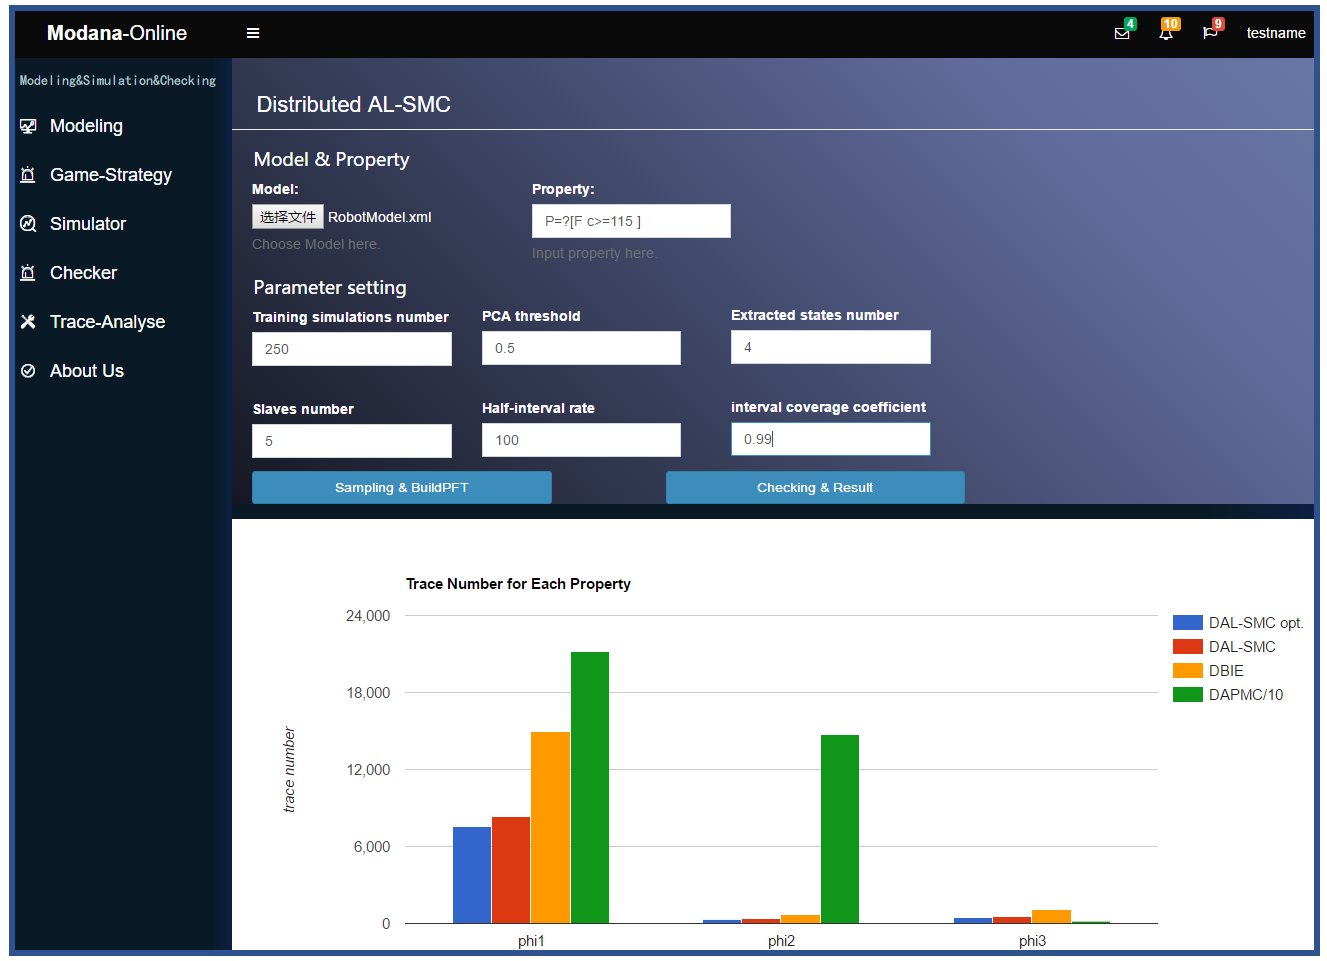
\includegraphics[width=3.2in,height=2.1in]{fig/system.png}}
	%\vspace{0.10in}
	\caption{The user interface of DAL-SMC.}\label{ui_dsmc}
\end{figure}

\subsection{Benchmark experiments}
Uppaal-SMC \cite{Bulychev2012UPPAAL} is a new version of UPPAAL which supports SMC and adopts many SMC algorithms (BHT \cite{jha2009bayesian},SPRT \cite{younes2006statistical}, BIE \cite{zuliani2013bayesian}, APMC \cite{herault2004approximate} etc.). In this paper, we model the benchmark with Uppaal-SMC, and then import the model (.xml) into our platform to verify the properties. Here, we use a simple benchmark to exhibit the distribution of traces in each slave and compare the probability partition between DAL-SMC with parameter optimization (DAL-SMC opt.) and DAL-SMC. Besides, two complex benchmarks are also introduced to compare the efficiency and accuracy among distributed BIE, DAL-SMC, DAL-SMC opt. and distributed APMC (DAPMC) which is a classical quantitative SMC algorithm.

\subsubsection{Train-gate}

A number of trains are approaching a gate on which there is only one track, gate controls the trains to avoid collisions, and restarts them when it is possible to make sure that trains will eventually cross the gate. Figure \ref{train} is the template of the train. Trains delay according to an exponential distribution and synchronize with the gate. The gate keeps track of the trains with an internal queue data structure as shown in Figure \ref{gate}.
\begin{figure*}[htbp]
\centering{
		\subfigure[Train]{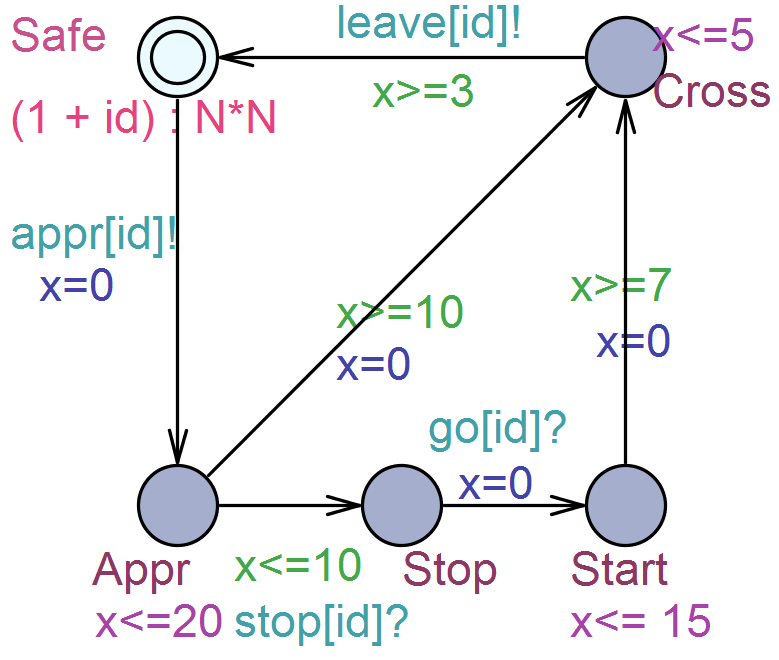
\includegraphics[width=2.0in,height=1.8in]{fig/train.png}
			\label{train}}
		\hfil
		\subfigure[Gate]{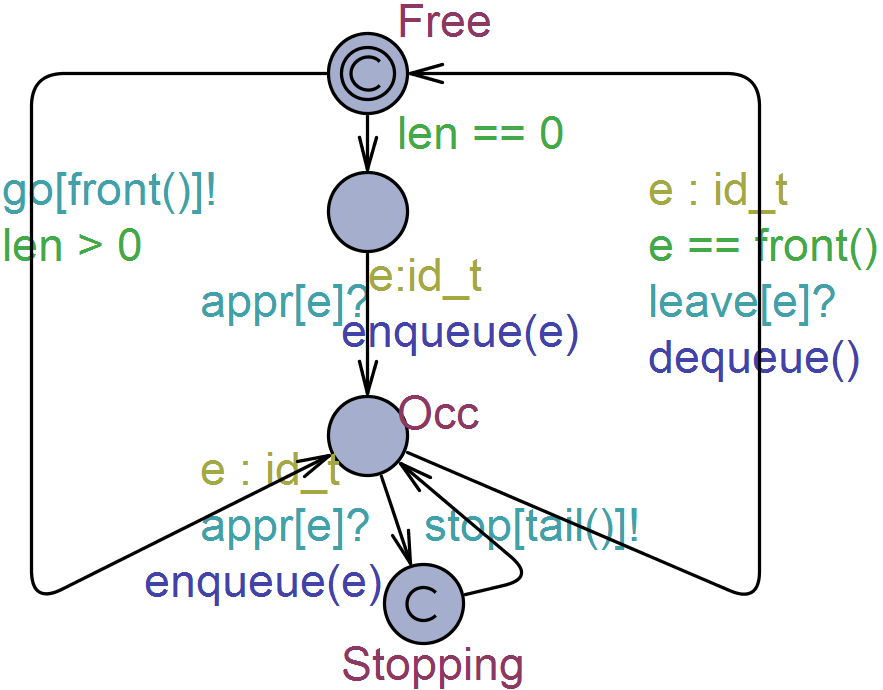
\includegraphics[width=2.5in,height=1.8in]{fig/gate.png}
			\label{gate}}
	\caption{The SHA templates for train-gate.}
	\label{ui_tg}
	}
\end{figure*}
We use Formula \ref{train-proba} to evaluate the probability of Train(0) crossing the gate:
\begin{equation}
P_{=?}(F^{\leq100}~Train(0).Cross)
\label{train-proba}
\end{equation}
\begin{figure}[htbp]
	\centering
	{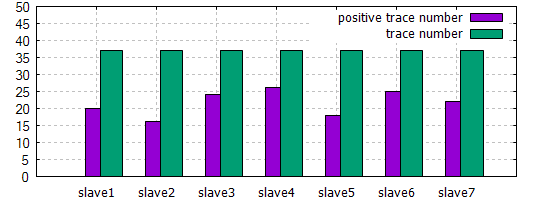
\includegraphics[width=3.2in,height=1.4in]{fig/trace-slave.png}}
	%\vspace{0.10in}
	\caption{Trace number of each slave}
   \label{trace-slave}
\end{figure}
The PBLTL property is used to evaluate the probability interval of Train(0) crossing the gate in 100 time units. The evaluation result is in [0.52707,0.626969] with half-interval size of $\pm0.05$ and interval coverage coefficient of 95\%. We plot the number of traces and satisfying traces of each slave in Figure \ref{trace-slave}. It shows that the slaves generate the same number of traces, however, the number of satisfying traces are not equal. Besides, in order to compare the probability partition between DAL-SMC and DAL-SMC opt, we plot the probability of each sub-space as shown in Figure \ref{BIE-pro}. Figure \ref{pronor} and Figure \ref{proopt} are the probability of each sub-space in DAL-SMC and DAL-SMC opt. respectively. We find that the probability distribution of DAL-SMC opt. is more evenly than that of DAL-SMC, therefore, the parameter optimization is effective. In the next subsections, we will use two complex CPS benchmarks to compare the performance of distributed BIE, DAL-SMC, DAL-SMC opt. and DAPMC.
\begin{figure*}[htbp]
\centering{
		\subfigure[DAL-SMC]{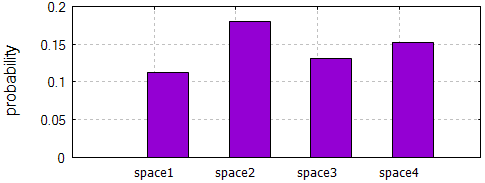
\includegraphics[width=3.0in,height=1.4in]{fig/pro.png}
			\label{pronor}}
		\hfil
		\subfigure[DAL-SMC opt]{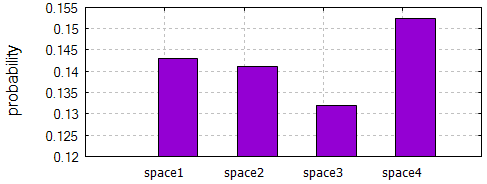
\includegraphics[width=3.0in,height=1.4in]{fig/pro-opt.png}
			\label{proopt}}
	\caption{Probability of each sub-space.}
	\label{BIE-pro}
	}
\end{figure*}

\subsubsection{Energy-aware building}
Energy-aware buildings play an important role in achieving an energy efficient society. The goal is to evaluate and compare the energy consumption of various control strategies with varying environmental settings. There are five SHA models: \emph{room temperature, heater, controller, weather} and \emph{user profile}. Figure \ref{ui_sb} shows the main SHA templates for energy-aware building. In Figure \ref{room}, the room needs to be heated when the temperature is lower than a threshold. The heater moves between locations "Off" and "On" based on the temperature thresholds $on[r]$ and $off[r]$, where r denotes the number of heated room. The central controller decides how to move the heater from one room to another room as shown in Figure \ref{controller}.

\begin{figure*}[htbp]
\centering{
		\subfigure[Room]{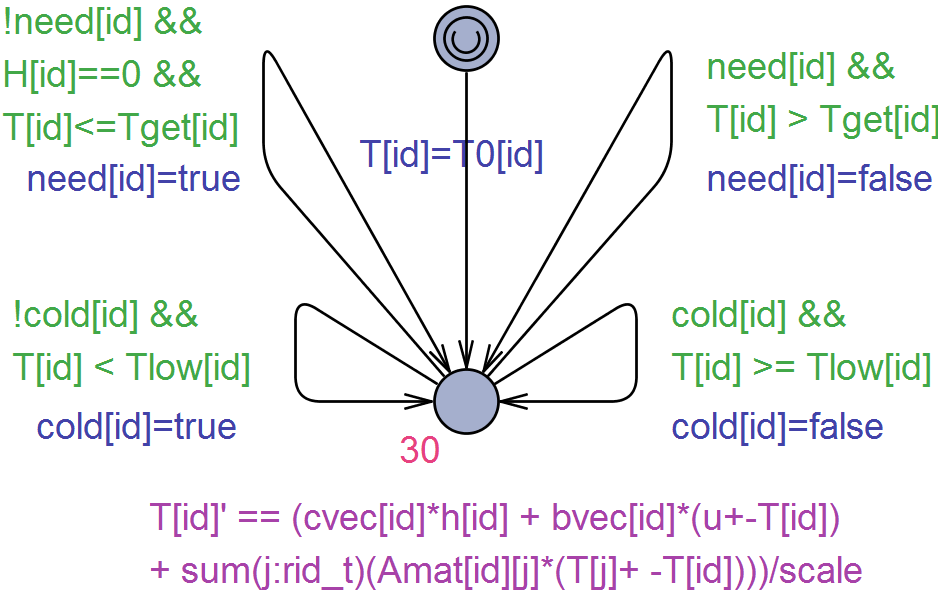
\includegraphics[width=1.8in,height=1.4in]{fig/room.png}
			\label{room}}
		\hfil
		\subfigure[Heater]{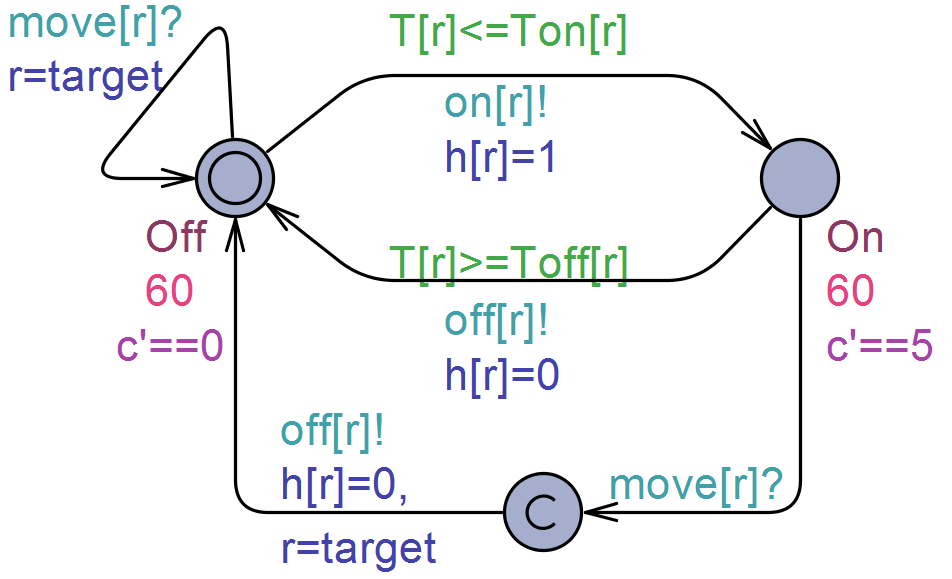
\includegraphics[width=1.8in,height=1.4in]{fig/heater.png}
			\label{heater}}
		\hfil
		\subfigure[Controller]{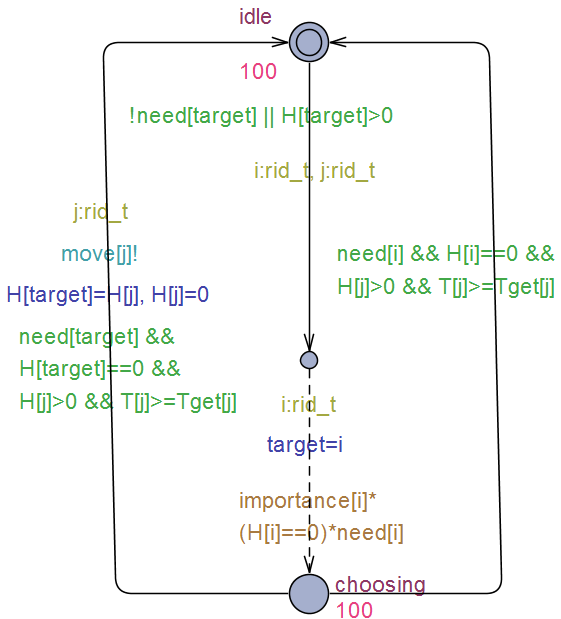
\includegraphics[width=1.5in,height=1.4in]{fig/strategy.png}
			\label{controller}}
	\caption{The main SHA templates for energy-aware building.}
	\label{ui_sb}
	}
\end{figure*}

The experiment has been performed on five slaves on a cluster with Intel Core(TM) i7-4790 (octa-cores at 3.6GHz) interconnected with infiniband. To compare the effciency and accuracy of the algorithms, three properties are verified, which are listed in Table \ref{tb:property}. $\delta$ and $c$ denotes half-interval size and interval coverage coefficient respectively.

\begin{table}[t]
	\renewcommand{\arraystretch}{1.2}
	\caption{Properties of energy-aware building}
	\label{tb:property}
	\centering
	\begin{tabular}{c c l}
		\hline
		~PID~ & $(\delta,c)$ & Property\\
		\hline
		$\phi_1$ & $(0.05,0.99)$ & $P_{=?}(F^{\leq48}~energy \geq 210)$ \\ 
		$\phi_2$ & $(0.01,0.99)$ & $P_{=?}(F^{\leq48}~discomfort \geq 15)$ \\
		$\phi_3$ & $(0.02,0.9)$ & 
		\tabincell{c}{$P_{=?}(F^{\leq48}~ discomfort \leq 15$ \\ $\wedge~energy \geq 170)$} \\
		\hline
	\end{tabular}
\end{table}

We execute each algorithm many times, and compare them in three aspects: the number of traces, time consumption and statistical error. In order to analyse the statistical error of algorithm, we verify the property with high interval coverage coefficient and small half-interval size to obtain the probability ($P_r$). We suppose $P_r$ is the true probability, therefore, the statistical error of each algorithm is $P_r - P_a$, where $P_a$ is the estimation of the true probability. Figure \ref{rs_sb} shows the number of traces, time consumption and statistical error of each algorithm.

\begin{figure*}[htbp]
\centering{
		\subfigure[Trace number of each algorithm]{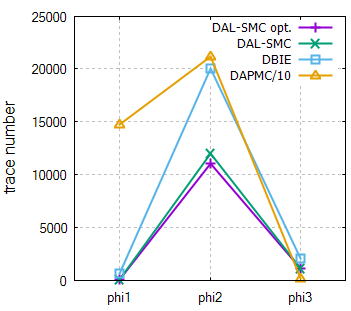
\includegraphics[width=2.0in,height=1.7in]{fig/sb-trace.png}
			\label{trace_sb}}
		\hfil
		\subfigure[Verification time of each algorithm]{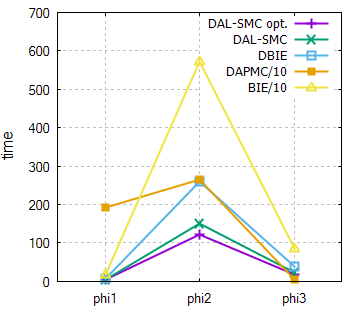
\includegraphics[width=2.0in,height=1.7in]{fig/sb-time.png}
			\label{time_sb}}
		\hfil
		\subfigure[Statistical error of each algorithm]{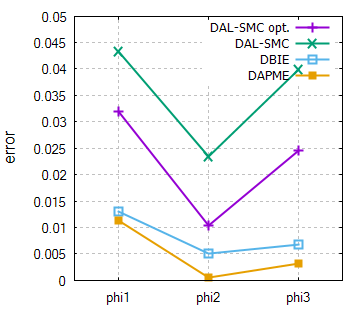
\includegraphics[width=2.0in,height=1.7in]{fig/sb-error.png}
			\label{error_sb}}
	\caption{Algorithms comparison with energy-aware building.}
	\label{rs_sb}
	}
\end{figure*}

Figure \ref{trace_sb} shows the trace number of energy-aware building benchmark generated by each algorithm. We can find that DAPMC algorithm needs 200000 traces to verify property $\phi_2$, however, distributing BIE (DBIE) algorithm only needs 20000 traces. DAL-SMC and DAL-SMC opt. need less traces (about 10000). The time consumption of each algorithm is shown in Figure \ref{time_sb}. The time consumption for verifying property $\phi_2$ with BIE algorithm is 6000 seconds, while it is around 250 seconds consumed by distributed BIE. DAL-SMC and DAL-SMC opt. consume less time. Figure \ref{error_sb} is the statistical error of each algorithm. The statistical error of DAPMC and distributed BIE are about 0.013 for verifying property $\phi1$. The statistical error of DAL-SMC and DAL-SMC opt are about 0.045 and 0.032 respectively. The detailed experiment results are listed in Table \ref{ta-rs}. 

\subsubsection{Robots path planning}

Robots path planning has attracted public attention these years \cite{LWAB10}. The basic goal of a mobile robot is to avoid collision with the moving obstacles, which move irregularly around the environment. As soon as the robot observes the moving obstacle, it will take actions immediately. Different actions consume different energy, so we use some variables to monitor the total energy consumption. Figure \ref{robot-ob} shows the main SHA templates for robot path planning.

\begin{figure*}[htbp]
\centering{
		\subfigure[Robot]{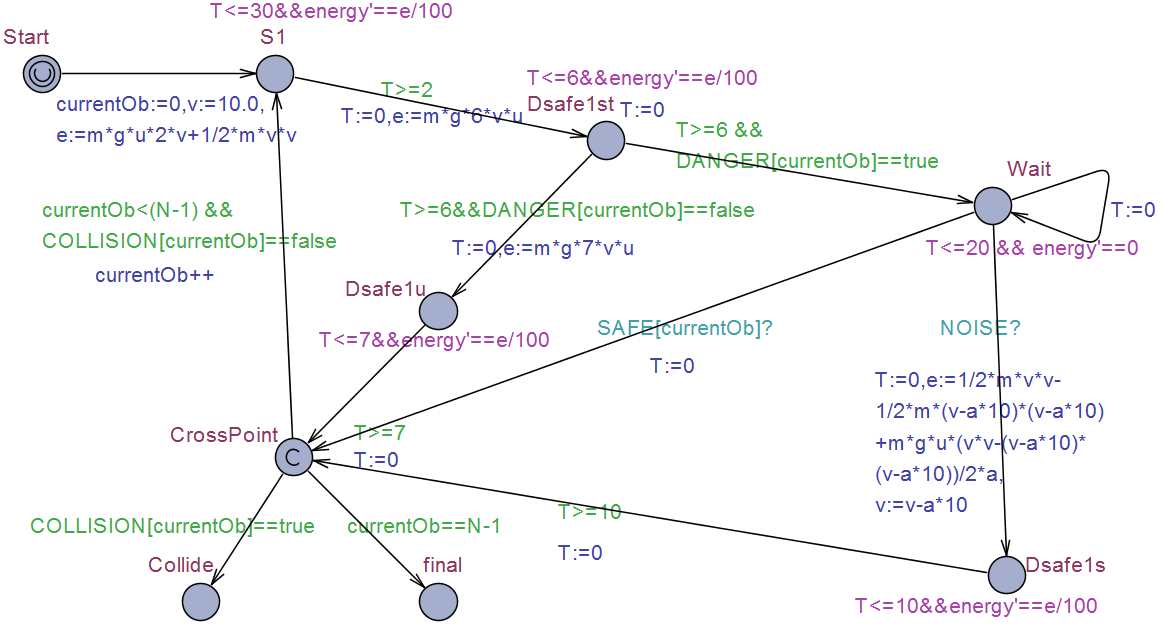
\includegraphics[width=3.0in,height=2.0in]{fig/robot.png}
			\label{robot}}
		\hfil
		\subfigure[Obstacle]{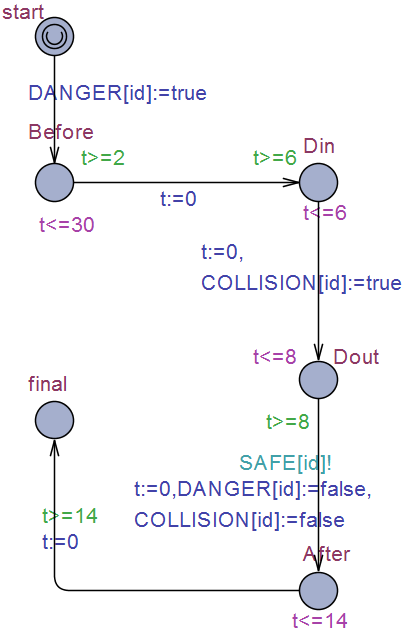
\includegraphics[width=1.5in,height=2.0in]{fig/obstacle.png}
			\label{obstacle}}
	\caption{The main SHA templates for robot path planning.}
	\label{robot-ob}
	}
\end{figure*}


\begin{figure*}[htbp]

\centering{
		\subfigure[Trace number of each algorithm]{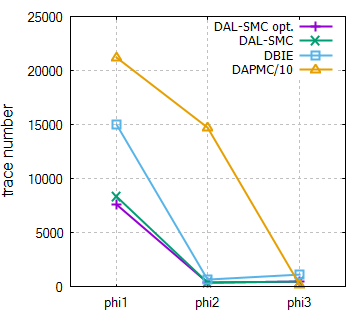
\includegraphics[width=2.0in,height=1.7in]{fig/ro-trace.png}
			\label{trace_ro}}
		\hfil
		\subfigure[Verification time of each algorithm]{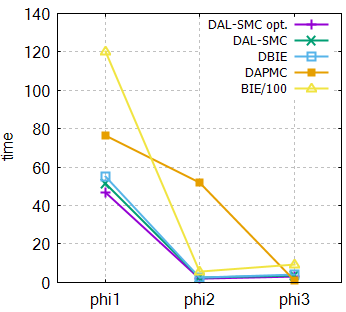
\includegraphics[width=2.0in,height=1.7in]{fig/ro-time.png}
			\label{time_ro}}
		\hfil
		\subfigure[Statistical error of each algorithm]{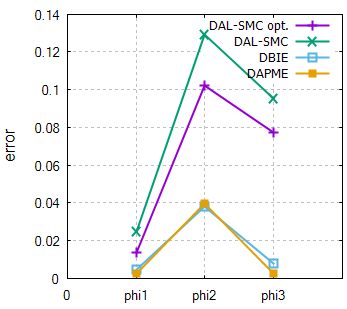
\includegraphics[width=2.0in,height=1.7in]{fig/ro-error.png}
			\label{error_ro}}
	\caption{Algorithms comparison with robots path planning.}
	\label{rs_ro}
	}
\end{figure*}


\begin{table}[t]
	\renewcommand{\arraystretch}{1.2}
	\caption{Properties of robots path planning}
	\label{tb:robot}
	\centering
	\begin{tabular}{c c l}
		\hline
		~PID~ & $(\delta,c)$ & Property\\
		\hline
		$\phi_4$ & $(0.01,0.99)$ & $P_{=?}(F^{\leq100}~robot.collision)$ \\ 
		$\phi_5$ & $(0.05,0.99)$ & $P_{=?}(F^{\leq100}~energy \geq 500)$ \\
		$\phi_6$ & $(0.02,0.9)$ & 
		\tabincell{c}{$P_{=?}(F^{\leq100}~robot.collision$ \\ $\wedge~energy \geq 500)$}\\
		\hline
	\end{tabular}
\end{table}


We also verify three properties $\phi_4$, $\phi_5$, $\phi_6$ for this benchmark as shown in Table \ref{tb:robot}. The experiment results are shown in Figure \ref{rs_ro}. 

In order to analyse the performance of SMC algorithms, the detailed data is listed in Table \ref{ta-rs}. Property $\phi_2$ is verified to illustrate the experimental results, we can conclude that: 

(i)DAPMC generates the most traces for verifying the property, while distributed BIE needs less traces compared with DAPMC. Furthermore, DAL-SMC reduces the number of traces (about 50\%) relative to distributed BIE.  In short, DAL-SMC is the most effective algorithm to generate traces.

(ii)The main time consumption of verification is generating traces (more than 90\%). DAPMC consumes most time, and DAL-SMC consumes less time compared with distributed BIE profitting from less traces. For the benchmark, we use 40 cores to implement distributed algorithms, and we find that the time consumption of BIE algorithm is nearly 25 times as much as distributed BIE which shows it is effective to improve the performance of SMC with distributed techniques. 

(iii)The statistical error of DAPMC and DBIE are similar. The error of DAL-SMC is bigger than that of DAPMC and DBIE due to use multi-BIE. Besides, we find that the error of DAL-SMC opt. is less than that of DAL-SMC. It shows that the parameter optimization method is effective. 

In general, DAL-SMC opt. generates less traces and consumes less time for verification with the help of distributed technology and AL-SMC technique. Meanwhile, the parameter optimization method reduces the statistical error of DAL-SMC to an acceptable range.

\begin{table*}
\caption{Experimental results}
\centering
\begin{tabular}{c c c c c c} 
        \hline  
        Algorithm & Property & Trace Number & Time consumption & Statistical Error\\
        \hline
        \multirow{6}{1.5cm}{DAPMC}  
                & $\phi1(0.05,0.99)$ &  147000&  1934.31&  0.0113\\ 
                & $\phi2(0.01,0.99)$ &  \textbf{211932} &  \textbf{2649.15} &  \textbf{0.0005}\\ 
                & $\phi3(0.02,0.9)$ &  1950&     38.05& 0.0032\\ 
                & $\phi4(0.01,0.99)$ &  211930&  76.282 &  0.0024\\ 
                & $\phi5(0.05,0.99)$ &  147550&  52.206&  0.0399\\ 
                & $\phi6(0.02,0.9)$ &  1850&     1.159& 0.0026\\     
        \hline 
        \multirow{6}{1.5cm}{DBIE}  
                & $\phi1(0.05,0.99)$ &  600&  7.895&  0.0131\\ 
                & $\phi2(0.01,0.99)$ &  \textbf{20000}&  \textbf{259.275} &  \textbf{0.0051} \\ 
                & $\phi3(0.02,0.9)$ &  2100& 38.057& 0.0068\\ 
                & $\phi4(0.01,0.99)$ & 15000&  55.281 &  0.0049\\ 
                & $\phi5(0.05,0.99)$ &  702&  2.483&  0.0382\\ 
                & $\phi6(0.02,0.9)$ &  1120& 4.226& 0.0078\\      
        \hline 
        \multirow{6}{1.5cm}{DAL-SMC}  
                & $\phi1(0.05,0.99)$ &  103&  5.685&  0.0433\\ 
                & $\phi2(0.01,0.99)$ &  \textbf{12000}&  \textbf{151.785} &  \textbf{0.0235} \\ 
                & $\phi3(0.02,0.9)$ &  1137& 22.841& 0.0399\\ 
                & $\phi4(0.01,0.99)$ &  8318&  41.68 &  0.0246\\ 
                & $\phi5(0.05,0.99)$ &  384&  2.32&  0.1295\\ 
                & $\phi6(0.02,0.9)$ &  520& 3.601& \ 0.0751\\      
        \hline 
         \multirow{6}{1.5cm}{DAL-SMC opt.}  
                & $\phi1(0.05,0.99)$ &  95.79&  4.65&  0.0319\\ 
                & $\phi2(0.01,0.99)$ &  \textbf{11040}&  \textbf{121.425} &  \textbf{0.0103}\\ 
                & $\phi3(0.02,0.9)$ &  1091& 18.73& 0.0246\\ 
                & $\phi4(0.01,0.99)$ &  7569&  36.512 &  0.0138\\ 
                & $\phi5(0.05,0.99)$ &  349&  1.81&  0.102\\ 
                & $\phi6(0.02,0.9)$ &  494& 3.171& 0.0575\\     
        \hline 
         \multirow{6}{1.5cm}{BIE}  
                & $\phi1(0.05,0.99)$ &  590&  175.44&  0.0121\\ 
                & $\phi2(0.01,0.99)$ &  \textbf{19586}&  \textbf{5730.67} &  \textbf{0.0047} \\ 
                & $\phi3(0.02,0.9)$ &  2040& 845.73& 0.0063\\ 
                & $\phi4(0.01,0.99)$ & 15400&  1202.467 &  0.0044\\ 
                & $\phi5(0.05,0.99)$ &  762&  55.221&  0.0352\\ 
                & $\phi6(0.02,0.9)$ &  1150& 91.98& 0.0069\\      
        \hline 
\end{tabular} 
\label{ta-rs}
\end{table*}


